\section{Why the tolerance must not decide what is discarded}\label{sec:failure}

Suppose that at some time every alternative $k$ has a box $\Lb_k\le\mub_k\le\Ub_k$ that contains its mean, as it will on the high-probability event constructed in Section~\ref{sec:method}. A certificate that $j$ $\epsb$-dominates $k$ is the inequality $\Ub_j\le\Lb_k+\epsb$, because it implies $\mub_j\le\Ub_j\le\Lb_k+\epsb\le\mub_k+\epsb$. The rule we first implemented, which we call \emph{$\epsb$-elimination}, discards $k$ as soon as some $j\ne k$ certifiably $\epsb$-dominates it. Two alternatives with equal means certifiably $\epsb$-dominate each other once their boxes are narrower than $\epsb$, and the rule would then discard both; it therefore needs a tie-break, and the natural one discards only the later alternative of a mutual pair in a fixed order of the alternatives. The following result shows that the rule fails even when every box contains its mean.

\begin{proposition}\label{prop:failure}
Let $\varepsilon_i=\varepsilon>0$ for all $i$, and suppose that every box contains its mean and has width at most $\eta$ in every objective, where $\eta>0$ is a constant depending on the instance.
\begin{enumerate}[label=(\alph*),leftmargin=*,itemsep=0pt]
\item (Three objectives.) Let $a<b<c$ with $\max(b-a,c-b)<\varepsilon<c-a$, and $\mub_1=(a,b,c)$, $\mub_2=(c,a,b)$, $\mub_3=(b,c,a)$. Then $\Pset=\{1,2,3\}$, no pair of alternatives is an $\epsb$-tie (mutual $\epsb$-dominance), and $\epsb$-elimination discards all three alternatives.
\item (Two objectives, tie-break.) Let $\mub_k=(x_k,y_k)$ with $x_1<x_2<x_3$, $y_1>y_2>y_3$, $x_3-x_1<\varepsilon$, $y_1-y_2<\varepsilon$, $y_2-y_3<\varepsilon$ and $y_1-y_3>\varepsilon$. Then $\Pset=\{1,2,3\}$, and $\epsb$-elimination discards all three alternatives, both without a tie-break and with the tie-break that keeps the earlier alternative in the order $1,2,3$.
\item (Two objectives, chain.) Let $\mub_1=(0.30,0.70)$, $\mub_2=(0.38,0.55)$, $\mub_3=(0.46,0.40)$, $\mub_4=(0.10,0.95)$ and $\varepsilon=0.1$. Then $\Pset=\{1,2,3,4\}$, no pair of alternatives is an $\epsb$-tie, and $\epsb$-elimination discards alternatives 1 and 2, after which no surviving alternative $\epsb$-covers alternative~1.
\end{enumerate}
\end{proposition}

The proof, in Section~\ref{S-sec:proof-failure} of the Supplementary Material, verifies the inequalities with margin $\eta$. Figure~\ref{fig:failure} draws the three instances. In (a) the certificates form a directed cycle, $1\to2\to3\to1$, in which each alternative is discarded by another that is itself discarded. In (b) a cycle with two objectives is impossible when every certificate is one-directional (a short argument is given in the Supplementary Material), but the tie-break creates one: alternative~1 keeps its place against~2 and~2 against~3, while~3 discards~1 one-directionally and the two ties discard~2 and~3. Another order of the alternatives would have saved alternative~2, so the conclusion depends on how the analyst happened to label the alternatives. In (c) nothing is lost entirely, but alternative~1 is now represented only by alternative~3, which is $2\varepsilon$ away in the first objective. Longer chains degrade the cover further.

\begin{figure}[t]
\spacingset{1}
\centering
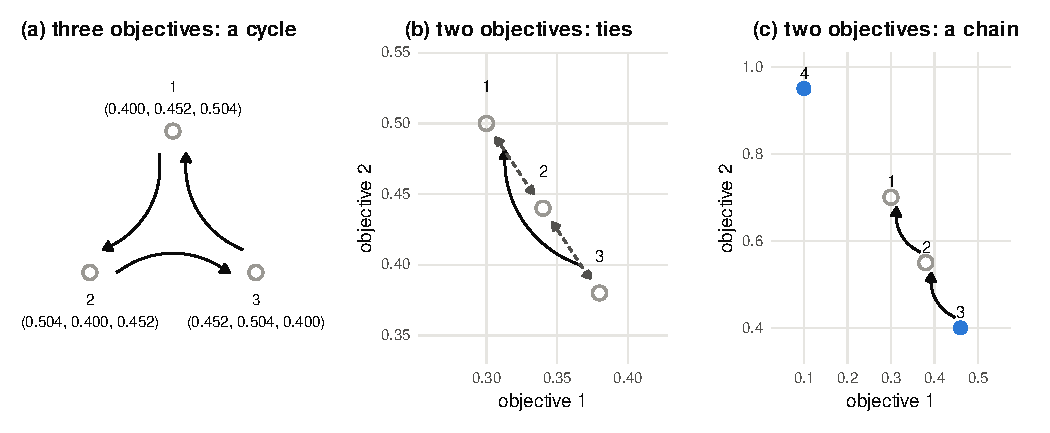
\includegraphics[width=\textwidth]{figures/fig1_failure.pdf}
\caption{The three instances of Proposition~\ref{prop:failure} with $\varepsilon=0.1$. Points are the mean vectors and arrows point from $j$ to $k$ when $j$ certifiably $\varepsilon$-dominates $k$; double-headed arrows are mutual certificates ($\varepsilon$-ties). (a) Three objectives, drawn in parallel coordinates: a cycle of one-directional certificates. (b) Two objectives: two ties and one one-directional certificate. (c) Two objectives: a chain $3\to2\to1$. Grey symbols are the alternatives that $\varepsilon$-elimination discards; in (a) and (b) it discards the whole Pareto set, which contains all alternatives. In all three panels, discarding by exact dominance discards nothing.}
\label{fig:failure}
\end{figure}

All three failures share a cause. A certificate that $j$ $\epsb$-dominates $k$ says something true about $j$ and $k$, but it is used to remove $k$ although nothing guarantees that $j$, or anything at least as good as $j$, will remain. Exact dominance does not have this defect: if $j$ certifiably dominates $k$ and $l$ certifiably dominates $j$, then $l$ certifiably dominates $k$, so the reason for a discard is never lost. The tolerance is still needed, but in the stopping rule rather than in the discarding rule. Proposition~\ref{prop:failure} does not depend on the confidence sequences, on the error level or on the allocation rule: it is a property of the decision rule applied to correct boxes. The simulation study in Section~\ref{sec:simulation} shows how often the failure occurs with noisy data.
